\subsection{The Server}
To construct the main sever, we chose java\cite{java} as our
programming language because of its multi platform abilities and the development
suit of eclipse\cite{eclipse} called swt\cite{swt} as our window-builder framework. We only used basic java libraries which came by default
with the eclipse IDE\cite{ide} environment, namely the
jdk7-openjdk\cite{open_jdk} package. 

When the Panstamp server is connected to the Java server, the latter takes the data given by the Panstamp server thanks to the RxTx library \cite{rxtx} and passes the information to the parser for processing. 

The server checks with an external timed thread the state of each known device.
This thread checks the current state of the device and, if necessary, sets the
state back to standby if too much time since the last change has passed. Therefore,
the thread compares the timestamp of the last state change with the current
time. Furthermore, it checks if the neighbor module is still detected by the device or not.

\begin{figure*}[ht]
	\centerline{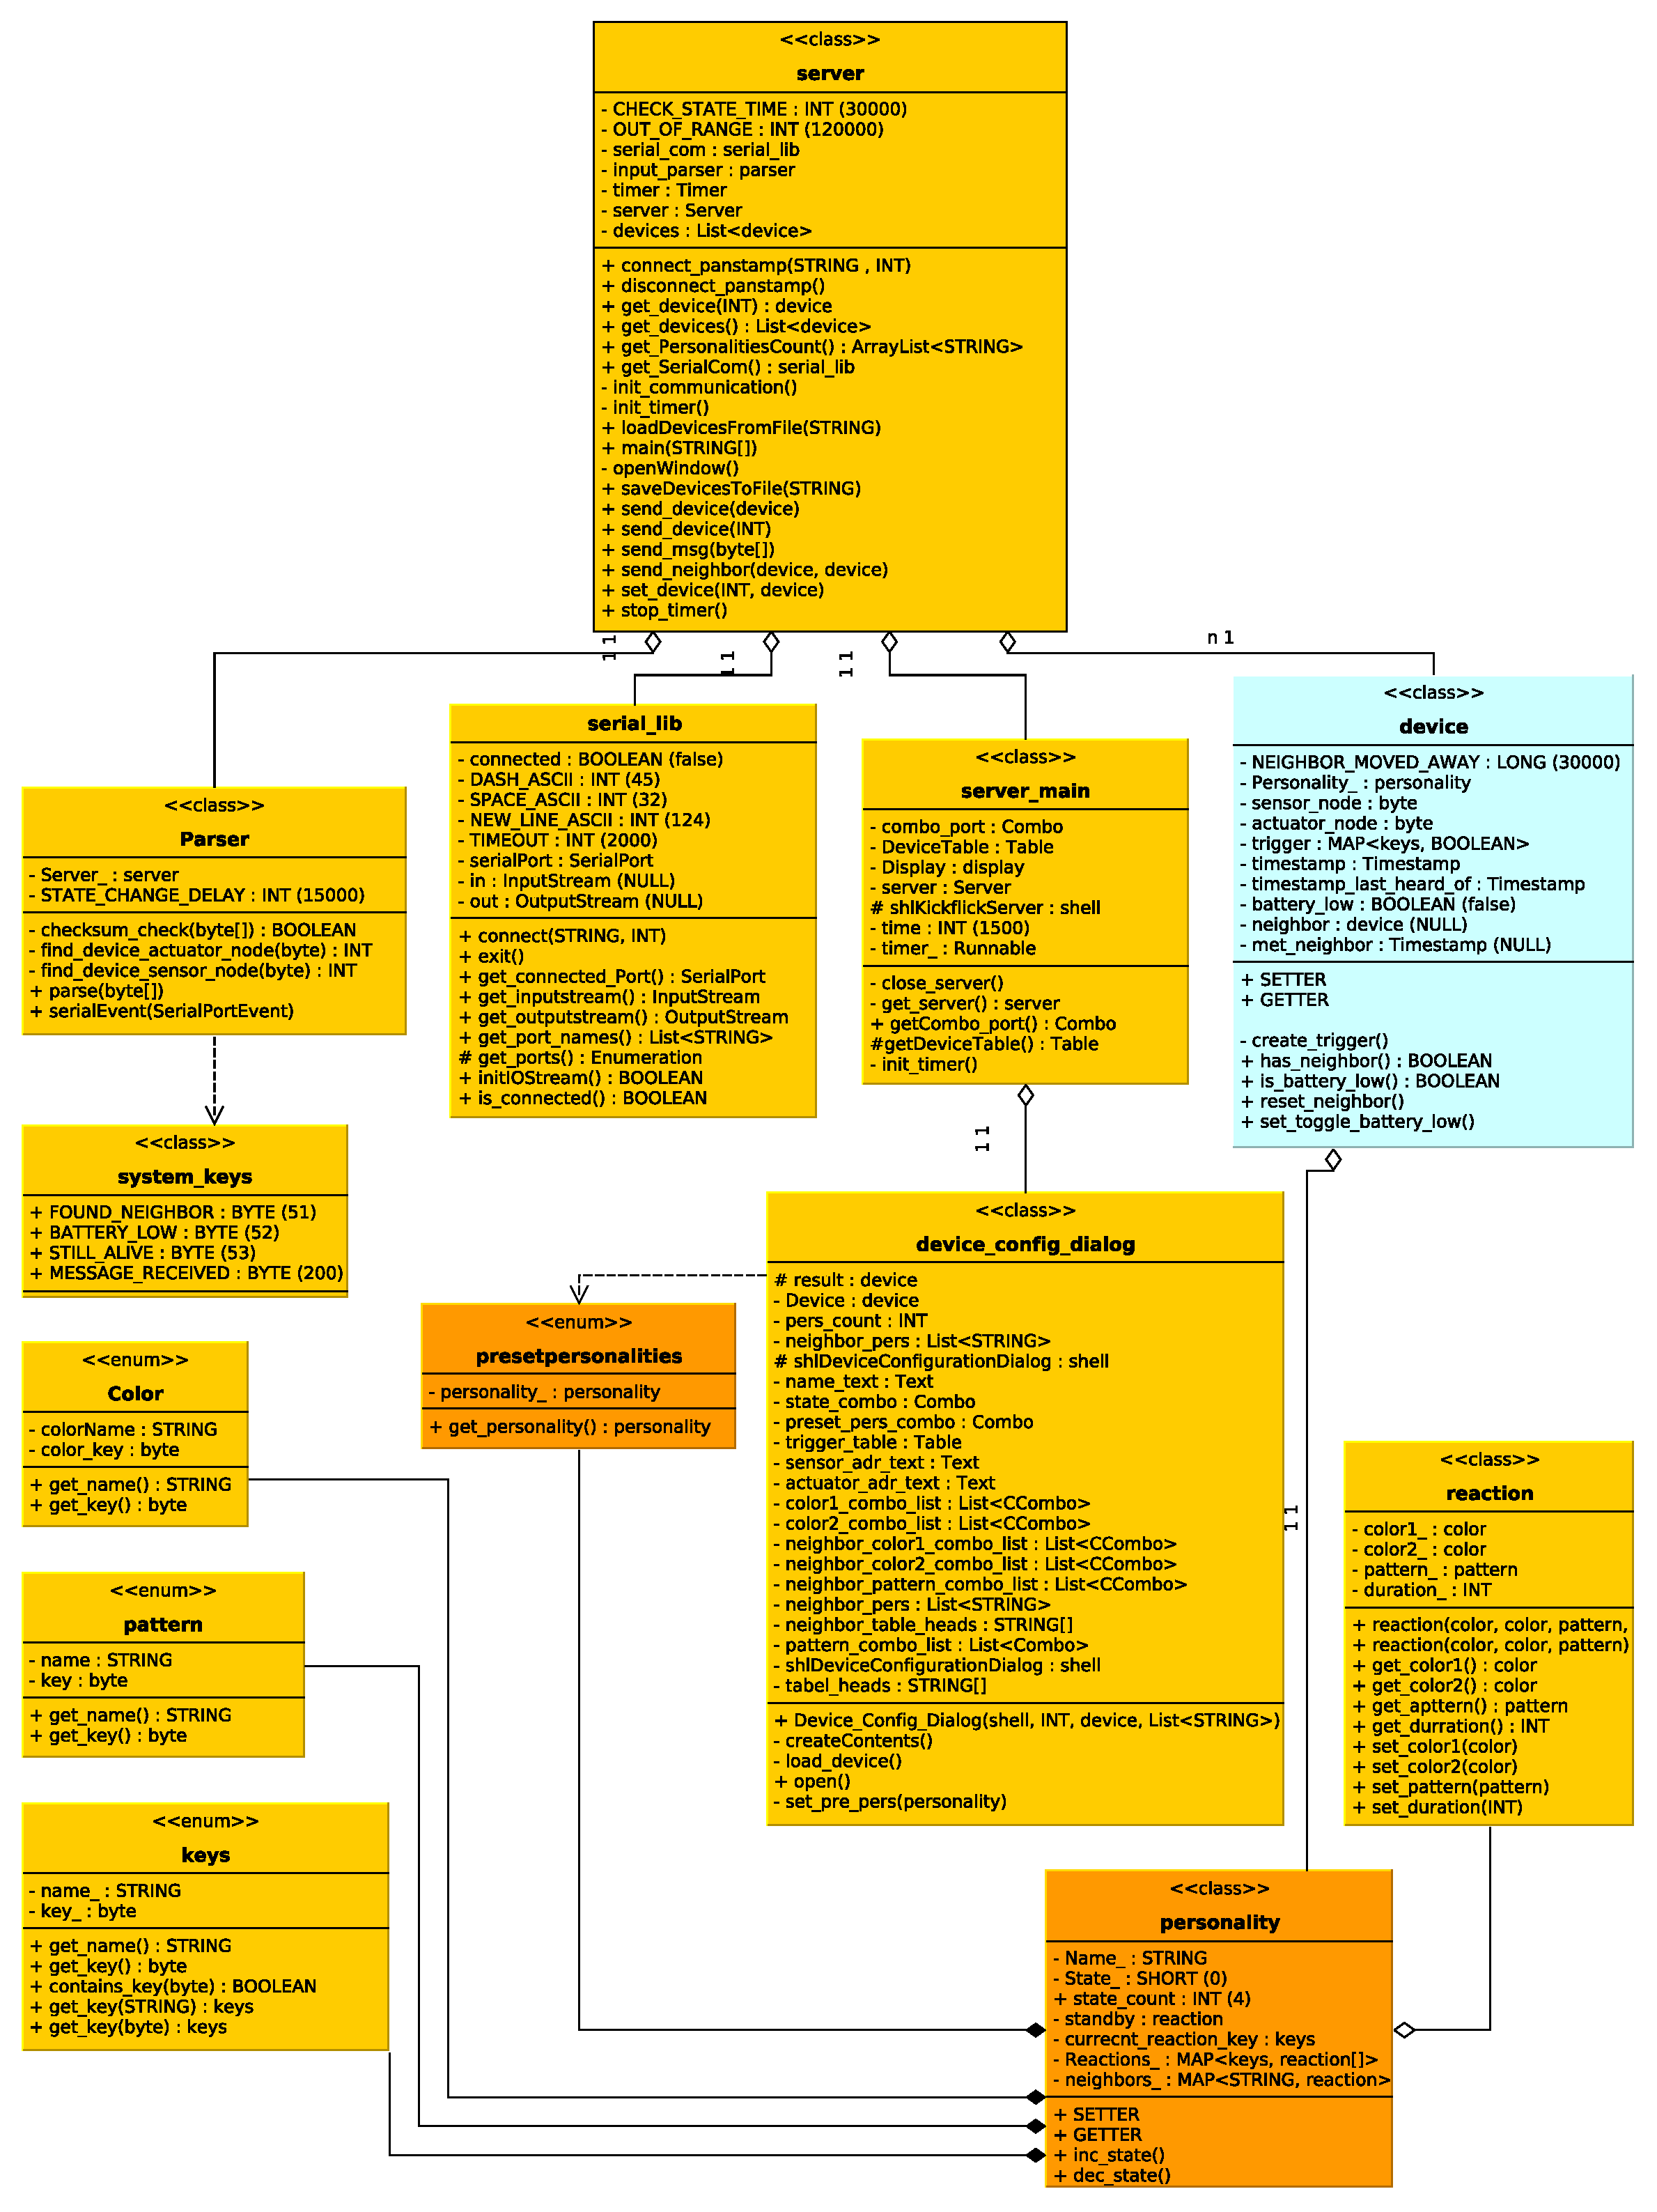
\includegraphics[width=\textwidth]{./graph/general.pdf}}
	\caption{UML Diagram of the Server Structure}
	\label{fig:server_uml}
\end{figure*}


\subsubsection{Panstamp-to-Java server message}
\label{sec:Panstamp-to-Java server message}
All messages sent by the Panstamp server to the Java Server contain four bytes. The message's length was set to a single value to achieve a better communication work-flow and to limit the communication's traffic to a minimum. Table~\ref{Panstamp-to-Java} shows the general structure of a message.


\begin{table}[h]
  \centering
  \begin{tabular}{ c | c | c | c }
    \hline
    \textbf{Byte 1} & \textbf{Byte 2} & \textbf{Byte 3} & \textbf{Byte 4} \\ [0.5ex]    
    \hline
    Sender's & Admin & Neighbor's Id| & Checksum  \\
    Id & Key & Dummy & \\
    \hline
  \end{tabular}
  \caption[Pamstamp-to-Java]%
          {Panstamp-to-Java server message's structure}
  \label{Panstamp-to-Java}
\end{table}

\begin{itemize}
\item \textbf{Sender's Id} is the Id of the network node that wants to report an event
\item \textbf{Admin Key} indicates the event reported by the entity. See table~\ref{Admin Keys} for further information.
\item \textbf {Neighbor's Id | Dummy } When the Admin Key equals NEARNODEEVENT, this byte contains the Id of the found neighbor node. For other keys this byte is ignored
\item \textbf {Checksum} This byte is the sum of bytes 1, 2 and 3 (modulo 256)
\end{itemize}

Table~\ref{Admin Keys} displays all the possible Admin Keys:

\begin{table}[h]
  \centering
  \begin{tabular}{ c | c }
    \hline
    \textbf{Name} & \textbf{Value}\\ [0.5ex]    
    \hline
    Shake Event & 31 \\
    Kick Event  & 32 \\
    Near Node Event & 51\\
    Low battery & 52\\
    In Range & 53\\   
    \hline
  \end{tabular}
  \caption[Admin Keys]%
          {Admin Keys}
  \label{Admin Keys}
\end{table}

\begin{itemize}
\item \textbf {Shake Event} indicates the entity has been shaken slightly so it is swaying
\item \textbf {Kick Event} means that the entity has been kicked or moved with a strong blow
\item \textbf {Near Node Event} signifies the entity has detected another entity which is really close to it
\item \textbf {Low Battery} warns the server that the entity's battery has to be recharged as soon as possible
\item \textbf {In range} indicates the server that the entity is still in range
\end{itemize}




\subsubsection{The Parser}
 
First, the parser checks whether the length of the package is exactly four bytes
and if the last byte, which is supposed to be a checksum summing the byte values
of every other bytes in the message, matches the checksum calculated by the
server. If everything is correct, the parser then searches for a known device in
the modules' list of the server. If it doesn't find a match, the parser will create a new device
with default settings. 

Once a device was found or created, the parser begins to compare the second byte of the message with the admin keys stored in the server data (see table~\ref{Admin Keys} ). First all system\_keys will be compared. For example if the received message contains a ''52'' as second byte, the parser will then recognize this as the ''the battery is low'' key and will toggle the boolean value battery\_low of the device to true. 
If no system key matched with the received one, the parser then checks the
reaction keys of the device itself. This check only happens if the device it not
currently engaged in a neighborhood relationship with another device and if the
time of the last received state changing message lays back a certain time. For
this checking and comparing procedure the device owns a map with all reaction
keys stored to it and a associated boolean value, representing the choice of
ignoring or reacting to the received key. If a appropriate key was found and
according to the boolean value a reaction should happen, then the state of the
devices personality will be increased and the new information about the pattern
and both colors, depending on the received event key, will be send to the
server-panStamp using the RxTx-library. 

No matter if a correct message lead to a state change or not, the device will
get a new timestamp to memorize the time of the last received message. If a
state change happend the device also gets a new timestamp revering to the time
the last state change happend.

\subsubsection{Device and Personality Structure}
The server itself and the according class holds a list of all known devices. Every lookup action depends on this list. The device class itself holds a instance of the personality class.
Devices can be seen as a representation of the hardware devices with the two panStamps in them. It refers to the hardware and therefor stores the Id's of the panStamps and timestamps of the last received message either one of the hardware device panStamps, a second timestamp of the last state change and a third timestamp of the last ''neighborhood meeting''. All those information are accessible through ''get'' functions as well as mostly modifiable through ''set'' functions.

The personality stores the reaction of a particular device depending on the
event keys, neighbors and the state of the device. For the purpose of reaction
to a certain event key the personality stores
a map for reactions with the acording keys as key and an array of reaction class
instances. If for example the parser received a message with an event key, the
reaction map will be searched for this particular key. If this key exsists in
the map the reaction array will be returned and the personality returns the
proper reaction fitting the current state. If the map holds no entry for the
gven key, the reaction map returns a default reaction array from with a fitting
reaction acording to the state will be returned. For this matter the default
map structre was extended to fit those requirements.
The possible reactions to each neighbor personality is also stored in a map. This
map contains the name of the personality as a key and one reaction as value. 
%The personality class stores information about the states of the personality and the according patterns and colors. This class also provides ''get'' and ''set'' functions to retrieve or change values. Additionally the personality class stores map object of all known personalities and the appropriate response in form of pattern and colors to every possible neighbor. If the device and therefor the personality encounter a unknown personality as a neighbor a default response will be send. 
%The neighbor map provides the ability to set reactions to neighbor personality, even if they don't exist yet.

Reactions represened by a class called reaction. This class stores information
about colos, patterns and the duration of one reaction. The duration determines
the time a reaction will be at least visible on the hardware.

To get the server and the project running without setting up every single device
by hand a enumeration for pre defined personalities was created. One can select
between each of those personalities. Once a pre defined personality is selected,
the previous personality of the current device will be overwritten. This
approach saves time. It is also possible to save the current devices to a file
so that they can be loaded again, for examlpe after restarting the server.
Therefor the classes device, personality and reaction are extending the
serialize class.

\subsubsection{Key Structure}
During the development we thought of keys, single byte values, to represent commands, messages, patterns and colors. To store these keys several enumerations were created to seperate related keys with their name and value depending on their usage.
We divided the keys in enumerations:
\begin{itemize}
    \item system
    \begin{itemize}
         \item stores basic keys for transmitting status information (e.g. ''low battery'')
				 \item enumeration: system\_keys
    \end{itemize}
    \item color
    \begin{itemize}
        \item stores byte values for every color hard coded to the actuator panStamp of the hardware device
				\item enumeration: color
    \end{itemize}
    \item pattern
    \begin{itemize}
        \item stores byte values for every pattern hard coded to the actuator panStamp of the hardware device
				\item enumeration: pattern
    \end{itemize}
    \item event key
    \begin{itemize}
        \item stores byte values for every possible action happening to the hardware device
				\item enumeration : keys
    \end{itemize}
\end{itemize} 

Every class or function referring to those values calls only the enumeration item by its name. The advantage of this approach is easier changing of single values as well as a quicker overview.
